\documentclass[10pt, letterpaper, titlepage]{article} % Set font here.
% Use 'article' for simple documents; use 'report' for larger documents with chapters;
% use 'book' for even larger documents with parts.
\usepackage[utf8]{inputenc}
\usepackage{geometry}
\usepackage{color,graphicx,overpic} 
\usepackage{fancyhdr} % header/footer stuff
\usepackage{amsmath,amsthm,amsfonts,amssymb}
\usepackage{mathtools} % more math stuff
\usepackage{siunitx} % for SI units, ex. $3.5 ~ \si{kg.s^{-2}}$
\usepackage{hyperref} % for hyperlinks
%\usepackage{apple_emoji}
\usepackage{multicol}
\usepackage{array}
\usepackage{float}
\usepackage{blindtext}
\usepackage{longtable}
\usepackage{scrextend}
\usepackage[font=small,labelfont=bf]{caption}
\usepackage[framemethod=tikz]{mdframed}
\usepackage{calc}
\usepackage{titlesec}
\usepackage{listings}
\usepackage[normalem]{ulem}

\usepackage{listings}
\usepackage{xcolor}

\DeclareMathOperator{\di}{d\!} % derivative operator symbol, ex. $\int f(x) \di x$
\newcommand{\Eval}[3]{\left.#1\right\rvert_{#2}^{#3}} % evaluation bar (ex. evaluating integral or $\Eval{F(x)}{0}{2}$)
\newcommand*\B{
\includegraphics[height=1.5em,valign=B,raise=-0.2em]{BigB.png}}
\newcommand*\fire{
\includegraphics[height=1.5em,valign=B,raise=-0.2em]{Fire.png}}

\definecolor{comment}{RGB}{140, 140, 140}
\definecolor{text}{RGB}{204, 204, 204}
\definecolor{string}{rgb}{0.58,0,0}
\definecolor{backcolour}{RGB}{27, 30, 39}
\definecolor{variable}{RGB}{244, 63, 78}

\lstdefinestyle{mystyle}{
    backgroundcolor=\color{backcolour},   
    commentstyle=\color{comment},
    keywordstyle=\color{variable},
    numberstyle=\tiny\color{text},
    stringstyle=\color{string},
    basicstyle=\ttfamily\footnotesize\color{text},
    breakatwhitespace=false,         
    breaklines=true,                 
    captionpos=b,                    
    keepspaces=true,                 
    numbers=left,                    
    numbersep=-10pt,                  
    showspaces=false,                
    showstringspaces=false,
    showtabs=false,                  
    tabsize=4
}

\lstdefinelanguage
   [x64]{Assembler}     % add a "x64" dialect of Assembler
   {morekeywords={	
   }} % etc.
   
\lstdefinelanguage[Motorola68k]{Assembler}{%
	morekeywords={	a0, a1, a2, a3, a4, a5, a6, a7, %
   					d0, d1, d2, d3, d4, d5, d6, d7, %
				   	ABCD,ADD,%
					ADDA,ADDI,ADDQ,ADDX,AND,ANDI,ASL,ASR,BCC,BLS,BCS,BLT,BEQ,BMI,BF,BNE,%
					BGE,BPL,BGT,BT,BHI,BVC,BLE,BVS,BCHG,BCLR,BRA,BSET,BSR,BTST,CHK,CLR,%
					CMP,CMPA,CMPI,CMPM,DBCC,DBLS,DBCS,DBLT,DBEQ,DBMI,DBF,DBNE,DBGE,DBPL,%
					DBGT,DBT,DBHI,DBVC,DBLE,DBVS,DIVS,DIVU,EOR,EORI,EXG,EXT,ILLEGAL,JMP,%
					JSR,LEA,LINK,LSL,LSR,MOVE,MOVEA,MOVEM,MOVEP,MOVEQ,MULS,MULU,NBCD,NEG,%
					NEGX,NOP,NOT,OR,ORI,PEA,RESET,ROL,ROR,ROXL,ROXR,RTE,RTR,RTS,SBCD,%
					SCC,SLS,SCS,SLT,SEQ,SMI,SF,SNE,SGE,SPL,SGT,ST,SHI,SVC,SLE,SVS,STOP,%
					SUB,SUBA,SUBI,SUBQ,SUBX,SWAP,TAS,TRAP,TRAPV,TST,UNLK},%
					sensitive=false,%
					morecomment=[l]*,%
					morecomment=[l] }[keywords,comments,strings]

\lstset{language=[Motorola68k]Assembler}
\lstset{style=mystyle}

\definecolor{mycolor}{rgb}{0, 0, 0}
  

\geometry{top=2.7cm,left=1.8cm,right=1.8cm,bottom=2.7cm}
\setlength{\headheight}{17pt}
\renewcommand{\baselinestretch}{1.5} 
\setlength{\parskip}{0.3cm}
\setlength{\parindent}{0.6cm}
\titlespacing\section{0pt}{12pt plus 4pt minus 2pt}{0pt plus 2pt minus 2pt}

\newcommand{\barrows}{\textcolor{blue}{\Longrightarrow}\quad}
\newcommand{\barrow}{\quad\textcolor{blue}{\Longrightarrow}\quad}  
\newcommand{\sumi}[1][1]{ \sum_{n={#1}}^{\infty} }
\newcommand{\limi}[1][n]{ \lim_{{#1}\to\infty} }

\title{\textbf{\Huge{
\begin{center}
Introduction to\\ Addressing Modes\\
\end{center}
}}}
\author{Benjamin Kong | 1573684\\Lora Ma ||||| 1570935\\ \\ECE 212 Lab Section H11}

\pagestyle{fancy}
\fancyhf{}
\rhead{Benjamin Kong \& Lora Ma}
\lhead{\textit{Introduction to Addressing Modes}}
\rfoot{Page \thepage}

\begin{document} 
\pagenumbering{gobble} 
\maketitle 
\thispagestyle{empty}
\tableofcontents 
\newpage
\pagenumbering{arabic}

\begin{multicols*}{2}


\section{Introduction}
As we learned in class, assembly language stores data in memory based on addresses. 
In this lab, we will investigate several different ways to address memory that is stored in memory. 
We also experiment with the differences between reading and writing to memory using these different addressing modes.

In part A of the lab, we wrote a program that adds adjacent contents of two arrays stored at different memory locations using three different methods to access memory:
\begin{itemize}
	\item Register Indirect With Offset,
	\item Indexed Register Indirect, and
	\item Postincrement Register.
\end{itemize}
The resulting array from adding the contents with each of the different addressing mode types are stored in three different locations before being output afterwards to the MTTY console. 
Note that for the first type of addressing mode (Register Indirect With Offset), we only perform the addition for the first 3 adjacent values to demonstrate that we understand this type of addressing.

In part B of the lab, we created a function that calculated the area underneath a curve given the data points using the trapezoidal rule. 
Using the data points stored in memory ($x$ and $y$ data points), it is mathematically trivial to calculate the area formed by the data points. 
Note that the distance between each $x$ data point is either one, two, or four units. 

\section{Design}
\subsection{Part A}
b

\subsection{Part B}
c

\section{Testing}
\subsection{Part A}
If properly implemented, part A should correctly add adjacent elements in two different arrays into a new resulting array, regardless of which of the three methods used. 
These methods were
\begin{itemize}
	\item Register Indirect With Offset,
	\item Indexed Register Indirect, and
	\item Postincrement Register.
\end{itemize}
For example, given two arrays $A = [A_0, A_1, ...]$ and $B = [B_0, B_1, ...]$ to add, our resultant array would be $C = [A_0 + B_0, A_1 + B_1, ...]$.
In order to test that our program functioned correctly, we ran our code against a test case (one of the DataStorage files) and compared our results to the expected results which were given to us by our TAs. 

Upon testing our program, it was evident that our program worked since our output matched what was expected and all methods used to add the arrays resulted in the same resultant array. Our screenshot of the MTTY terminal output is included in the appendix.

\subsection{Part B}
If properly implemented, part B should correctly calculate the area under a curve given a set of data points with $x$ and $y$ coordinates. We use the trapezoidal rule to accomplish this: we sum up the area of the trapezoid between each point from the first point to the last point and achieve the area under the graph. 

In order to determine if our program actually does this correctly, we ran our code against several test cases provided on eClass given in the form of DataStorage files and compared our output to the expected output provided to us. 

Upon testing our program, it was evident that our program worked since the areas that we found for each test case corresponded to the expected output. Our screenshot of the MTTY terminal output is included in the appendix.

\section{Questions}
\textit{What are the advantages of using the different addressing modes covered in this lab?}

Let ``Register Indirect with Offset" be mode 1, ``Indexed Register Indirect" be mode 2, and ``Postincrement Register" be mode 3. 
An obvious advantage mode 2 and mode 3 have over mode 1 is that since we are essentially able to loop until the array is finished, we can input an array of any size we wish rather than hard-coding each iteration of the loop. 
It is also significantly less tedious to implement mode 2 and mode 3 since significantly less code is needed when using a loop-like structure. 

Upon comparing mode 2 and mode 3, the difference is less pronounced. 
Mode 2 is slightly more complicated than mode 3 since mode 2 requires the coder to keep track of the address offset using another variable, while mode 3 automatically increments the address to the next location in memory each time the loop executes, removing the need for the coder to keep track of the current offset.

\textit{If the difference between the X data points are not restricted to be either one, two, or four units, how would you modify your program to calculate the area?}

\textit{From the data points, what is the function $y = f(x)$? What is the percent error between the theoretical calculated area and the one obtained in the program? Calculate all 3 functions.}

From DataStorage4, it is evident that the function is $f(x) = x^2$, and the data points given indicate that the range we are interested in is $[0, 50]$. Therefore, the actual area under the graph is given by
\begin{equation}
	A_1 = \int_0^{50} x^2 \di x = \dfrac{125000}{3} \approx 41666.666.
\end{equation} 
Our program output the value of 41675. Therefore, calculating error, we have
\begin{equation}
	\epsilon_1 = \dfrac{41675 - 41666.666}{41666.666} \cdot 100\% = 0.02\%. 
\end{equation}

From DataStorage5, it is evident that the function is again $f(x) = x^2$, and the data points given indicate that the range is $[0, 80]$. Therefore, the actual area under the graph is given by
\begin{equation}
	A_2 = \int_0^{80} x^2 \di x = \dfrac{512000}{3} \approx 170666.666.
\end{equation} 
Our program output the value of 170710. Therefore, calculating error, we have
\begin{equation}
	\epsilon_2 = \dfrac{170710 - 170666.666}{170666.666} \cdot 100\% \approx 0.02539\%. 
\end{equation}

From DataStorage6, it is evident that the function is again $f(x) = x^2$, and the data points given indicate that the range is $[0, 110]$. Therefore, the actual area under the graph is given by
\begin{equation}
	A_3 = \int_0^{110} x^2 \di x = \dfrac{1331000}{3} \approx 443666.666.
\end{equation} 
Our program output the value of 443843. Therefore, calculating error, we have
\begin{equation}
	\epsilon_3 = \dfrac{443843 - 443666.666}{443666.666} \cdot 100\% \approx 0.03974\%. 
\end{equation}

\section{Conclusion}
g


\end{multicols*}

\newpage

\section{Appendix}
\subsection{Part A MTTY Screenshots}
\begin{figure}[H]
   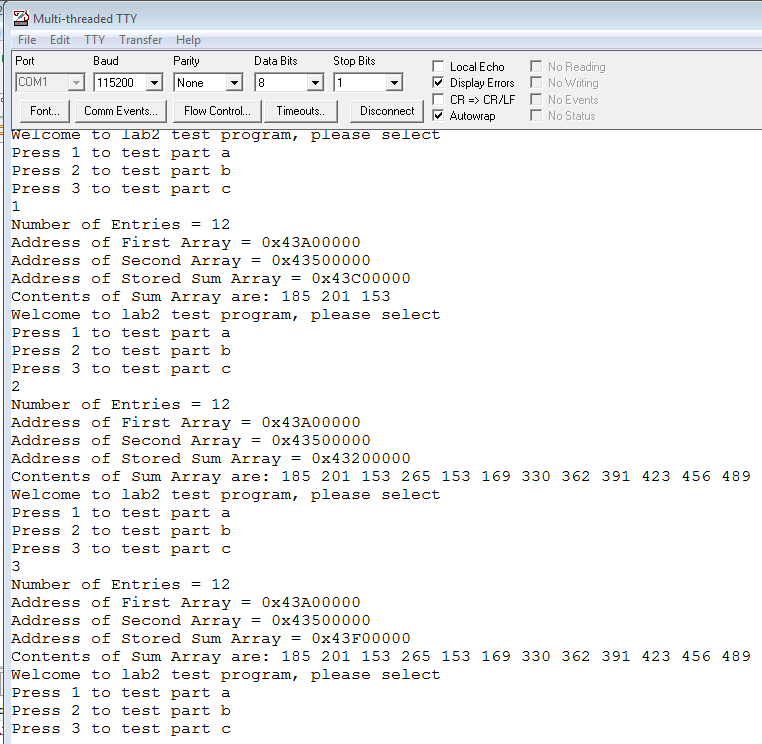
\includegraphics[width=0.52\textwidth]{mttypartA.png}
   \centering  
   \caption{Screenshot of MTTY output for part A.} 
   \label{figure:4}
\end{figure}

\subsection{Part B MTTY Screenshots}
\begin{figure}[H]
   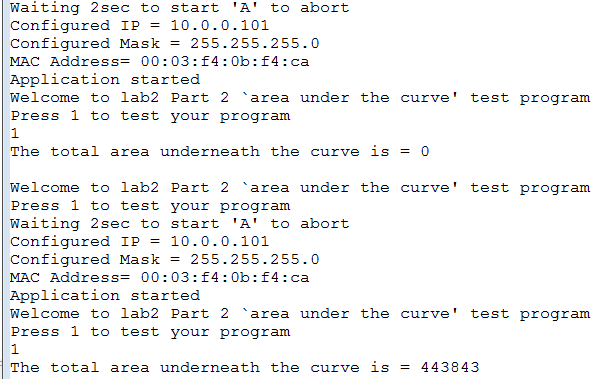
\includegraphics[width=0.45\textwidth]{mttypartB.png}
   \centering  
   \caption{Screenshot of MTTY output for part B.} 
   \label{figure:5}
\end{figure}

\subsection{Part A Assembler Code}
\begin{lstlisting}
	/*Part A **********************************************************/
	MOVEA.L #0x43000000, %a1 
	MOVE.L (%a1), %d3 /* d1 is the size of our array*/
	MOVEA.L #0x43000004, %a1
	MOVEA.L (%a1), %a2  /* address of first array */
	MOVEA.L #0x43000008, %a1
	MOVEA.L (%a1), %a3 /* address of second array */
	MOVEA.L #0x4300000C, %a1 
	MOVEA.L (%a1), %a4 /* where to store adjacent sums */
	
	MOVE.L (%a2), %d1 /* make a copy of first array value */
	MOVE.L (%a3), %d2 /* make a copy of second array value */
	ADD.L %d1, %d2 /* add first array value and second array value and put result into d2*/
	MOVE.L %d2, (%a4) /* move added value into address at a4 */
	
	MOVE.L 4(%a2), %d1 /*increment first array index and move new value into d1*/
	MOVE.L 4(%a3), %d2 /*increment second array index and move new value into d2*/
	ADD.L %d1, %d2 /*add values together*/
	MOVE.L %d2, 4(%a4) /*put added value into incremented array a4*/
	
	/*repeat above process*/
	MOVE.L 8(%a2), %d1 
	MOVE.L 8(%a3), %d2
	ADD.L %d1, %d2
	MOVE.L %d2, 8(%a4)
	
	/*Part B **********************************************************/
	
	MOVE.L #0, %d2  /* Store 0 into d2*/
	
	MOVEA.L #0x43000010, %a1 
	MOVEA.L (%a1), %a4 /*store address for result array*/
	
	loop_partB:
	CMP.L %d2, %d3 /*compare zero and d3 */
	BEQ next /* exit part B*/
	
	MOVE.L (%a2, %d2*4), %d1 /* add 4 to d2 and add to a2. Store value in d1 */
	ADD.L (%a3, %d2*4), %d1 /* Add d2 with 4, a3 and d1. Store value in d1 */
	MOVE.L %d1, (%a4, %d2*4) /* move the value of d1 into the value of d2+4+a4*/
	ADDI.L #1, %d2 /* Add 1 to d2*/
	BRA loop_partB /* loop */
	
	/*Part C **********************************************************/
	
	next:
	
	MOVEA.L #0x43000014, %a1 /*intialize value of a1*/
	MOVEA.L (%a1), %a4 /*initialize a4 with value at a1*/
	
	loop_partC:
	CMPI.L #0, %d3 /*compare d3 to 0*/
	BEQ exit /* if equal, exit */
	
	MOVE.L (%a2)+, %d1 /*put value of first array value into d1 and increment a3*/
	ADD.L (%a3)+, %d1 /* add value in seond array to d1 and increment a3*/
	MOVE.L %d1, (%a4)+ /* move value in d1 to array with results and increment the array */
	SUBI.L #1, %d3 /*subtract 1 from d3*/
	BRA loop_partC
	
	exit:
	
	/*End of program **************************************************/
\end{lstlisting}

\subsection{Part B Assembler Code}
\begin{lstlisting}
	/*Write your program here******************************************/
	MOVEA.L #0x43000000, %a1 
	MOVE.L (%a1), %d3 /* load value for data points at address a1 into d3*/
	
	MOVEA.L #0x43000004, %a1
	MOVEA.L (%a1), %a2 /*load array for x points in a2*/
	
	MOVEA.L #0x43000008, %a1
	MOVEA.L (%a1), %a3 /*load array for y points in a3*/
	
	MOVEA.L #0x43000010, %a1
	MOVEA.L (%a1), %a4 /*load results array in a4*/
	
	CLR.L %d2 /*clear d2*/
	
	loopVals:
	CMPI.L #1, %d3 /* compare 1 to data point */
	BEQ exit /* if equal, go to exit */
	
	SUBI.L #1, %d3 /*reduce counter by 1*/
	
	/* Load x vals, calculate delta x */
	MOVE.L 4(%a2), %d0
	SUB.L (%a2)+, %d0
	
	/* Load y vals, calculate sum of y */
	MOVE.L 4(%a3), %d1 /* increment y array and put new val into d1 */ 
	ADD.L (%a3)+, %d1 /* post increment a3 after adding current a3 val to d1*/
	
	loop_X:
	CMPI.L #1, %d0 /*compare value 1 with d0*/
	BEQ area /*if equal, calculate area*/
	LSR.L #1, %d0 /*logical shift right by 1 in d0*/
	LSL.L #1, %d1 /*logical shift left by 1 in d1*/
	BRA loop_X
	
	area:
	ADD.L %d1, %d2 /*add d1 and d2*/
	BRA loopVals 
	
	exit:
	LSR.L #1, %d2 /* divide by 2 */
	MOVE.L %d2, (%a4) /* store in results */
	
	/*End of program **************************************************/
\end{lstlisting}

\end{document}
